\documentclass[12pt]{article}

\usepackage{graphicx}
\usepackage[subpreambles=true]{standalone}
\usepackage{import}
\usepackage{float}


\begin{document}
\pagenumbering{gobble}
\linespread{1.0}
\begin{titlepage}
	\begin{center}
		\large{University of Puerto Rico\\
			Mayagüez Campus\\
			\vspace{\baselineskip}
			Department of Electrical and Computer Engineering}\\
		\vspace{5\baselineskip}
		\Huge{\underline{M.O.S.I.S U.I 2.0 Progress Report}\\}
		\vspace{\baselineskip}
		\large by\\
		Fabio J. Matos Nieves\\
		Eduardo S. Miranda Figueroa\\
		\normalsize
		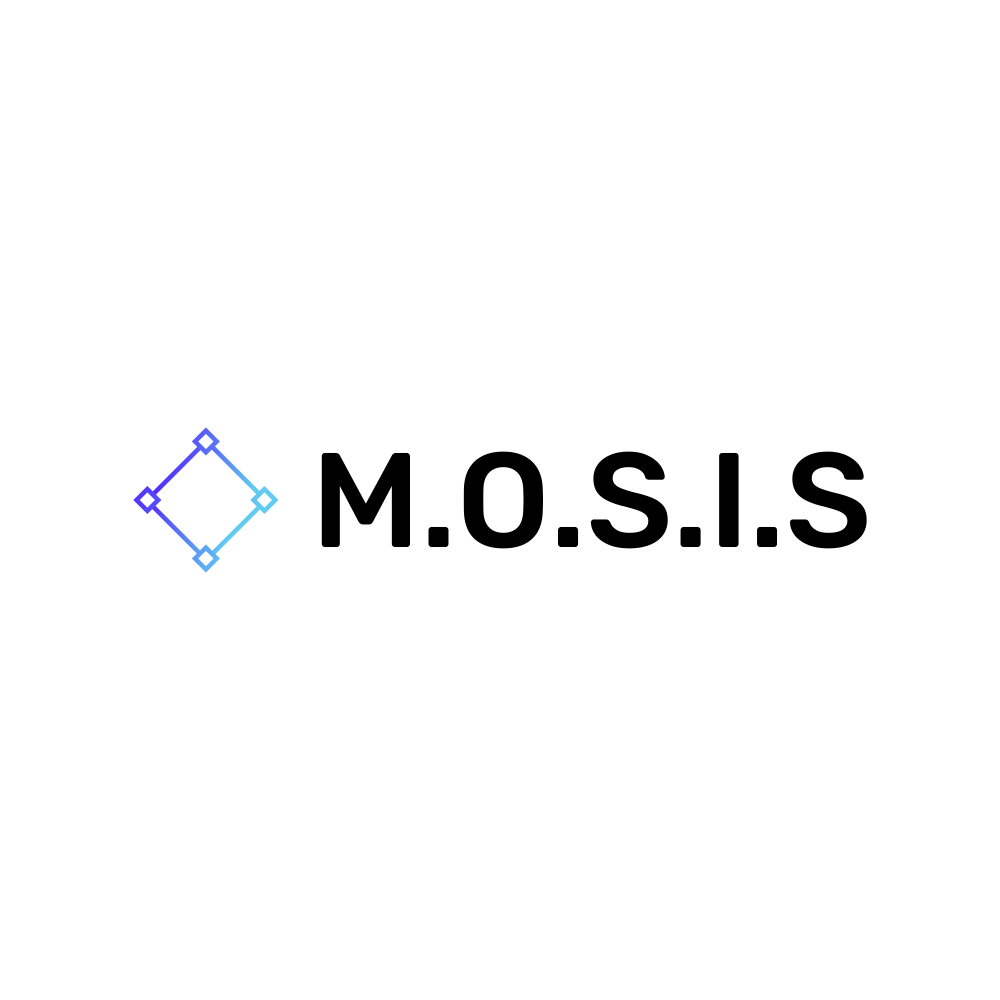
\includegraphics[scale=0.15]{../../M.O.S.I.S Logo/default.png}\\
		\vspace{4\baselineskip}
		\large
		For: Nayda Santiago\\
		Course: ICOM 5047, section 016\\
		Date: September 14, 2023\\
		\normalsize

	\end{center}
\end{titlepage}
\section*{Executive Summary}
\pagenumbering{roman}
\tableofcontents
\pagenumbering{arabic}
\section{Introduction}
The Marine Operated Stereoscopic Imaging System (M.O.S.I.S) is a device created by David M. Repollet Otero along with Manuel A. Jimenez Cedeno in order to study marine life \textit{in situ} in stereoscopic vision while capturing environmental conditions such as temperature, pH, pressure and dissolved oxygen. As of November 27, 2023, the microscope itself has a fully completed user interface capable of capturing various kinds of still photography and videos. However, at its core, the M.O.S.I.S microscope is an embedded system running a Raspberry Pi 4b, meaning that processing speed and memory are both severely limited. But not only is processing power limited, but the device itself will be deployed in an extremely hostile environment, where the microscope can be destroyed at a moments notice. Even more so, the microscope does not provide the means to recover the captured data nor does it provide the means to analyses and present the data to the user. The host software for the M.O.S.I.S microscope aims to backup the data captured by the M.O.S.I.S microscope, analyses the data captured by the microscope and generate reports based on the captured data.\\
\subsection{System Requirements}
\subsubsection{Domain Requirements}
\begin{itemize}
	\item The system-to-be must allow the backup of the M.O.S.I.S project Raspberry Pi's operating system.
	\item The system-to-be must allow the backup of the images captured by the M.O.S.I.S microscope Raspberry Pi.
	\item The system-to-be must have a database that stores the media captured by the M.O.S.I.S microscope Raspberry Pi.
	\item The system-to-be must have a database that stores the sensor data captured by the M.O.S.I.S microscope Raspberry Pi.
	\item The system-to-be must create a stereoscopic image from the media captured by the M.O.S.I.S microscope Raspberry Pi.
	\item The system-to-be must have the means to pre-configured the type of media capture before deployment in the field.
	\item The system-to-be must tag the media captured the M.O.S.I.S Raspberry Pi with the information stored in the database.
	\item The system-to-be must analyze the captured media for bleaching estimates.
	\item The system-to-be must create reports from the captured media.
\end{itemize}
\subsubsection{Interface Requirements}
\begin{itemize}
	\item The system-to-be's database must contain image information that includes:
	      \begin{itemize}
		      \item Left Camera Image
		      \item Right Camera Image
		      \item Stereoscopic Image
		      \item Left Threshold Image
		      \item Right Threshold Image
		      \item Time Stamp
		      \item Temperature
		      \item Ph
		      \item Pressure
		      \item Dissolved Oxygen (DO) Content
	      \end{itemize}
	\item The system-to-be must have a home page where there is a preview of all images currently within the database.
	\item The system-to-be must create an individual page for each entry within the database.
\end{itemize}
This report is organized in the following parts:
\begin{enumerate}
	\item Introduction
	\item Design Criteria and Design Specifications
	\item Methods and approach to the solution
	\item Market overview
	\item Results, and impact of the project
	\item Conclusions and Future Work
	\item Bibliographic References
	\item Appendix
\end{enumerate}
\section{Design Criteria and Specifications}
\subsection{System Specifications}
\begin{itemize}
	\item Backs up M.O.S.I.S microscope media data via SSH
	\item Generates stereoscopic images or video from left and right cameras.
	\item Tags stereoscopic media with the sensor data and time stamp associated with that entry.
	\item Generate threshold images from captured media.
	\item Allows searching by ID, shot type, illumination type and date.
	\item Exports either whole database or searched media entries to a PDF report.
	\item Creates compressed backups of M.O.S.I.S microscope operating system.
	\item Officially supports Windows and Linux operating systems.
\end{itemize}
\subsection{Design Criteria}
The main design criterion for the host software was to create a set of user friendly utilities that:
\begin{itemize}
	\item Abstracts and automates the process of interacting with the M.O.S.I.S microscope as much as possible.
	\item Is usable by marine biologist end users.
	\item Is reliable enough to backup and analyze the data from the M.O.S.I.S microscope for the lifetime of the device
	\item Is free and open source.
\end{itemize}
These design criteria are in part due to the target users of the M.O.S.I.S microscope, those being, marine biologist researchers. These researchers know how to analyze the captured data and to draw conclusions from said data, but most of them lack the expertise to use complex computer software, especially ones designed for computer scientists and engineers. Thus, with these design criterion in mind, the host software design process was applied in the following ways:
\begin{enumerate}
	\item Minimize interaction with the command line as much as possible.
	\item Automate the installation of dependencies as much as possible.
	\item Web browser based.
	\item Streamline the process of backing up the captured media and microscope operating system.
	\item Friendly and modern user interface design.
	\item Automate the process of data analysis.
	\item Streamline the process of data export.
	\item Seamless integration between the host machine and the Raspberry Pi.
\end{enumerate}
\subsection{Analysis of alternatives}
Given that the term ``host software'' and the design criteria are rather broad, this gives us a lot of possible and viable alternatives for a design. To start we need to first identify what are the possible ways of creating a user interface for this piece of software. There are 3 main approaches used in modern software design for making user interfaces:
\begin{enumerate}
	\item Command Line Interface (CLI)
	\item Terminal User Interface (TUI)
	\item Graphical User Interface (GUI)
\end{enumerate}
Both the command line and terminal interfaces utilize a terminal to display information and interact with the user but in distinct ways. CLI applications use command line parameters within a terminal to have differing functionality within the application and most require very little interaction from the user. A TUI application also runs within a terminal but are more akin to GUI applications where graphics and text are shown to the user and they can navigate through the application and require user integration like most GUI applications. Graphical user interfaces are traditional and modern way of interaction with software, where images, text, video, and various forms of multimedia are displayed to the user within a native interface or a web browser. Given that the end users for the host software are marine biology researchers, they are not accustomed to use the terminal as a means of using their computer, thus we can discard both command line and terminal user interfaces and chose a to make a Graphical User Interface.\\
Given that we are making a graphical user interface application, this now begs the question, what alternatives do we have at our disposal to make a graphical user interface? In modern software development, there are 3 main paradigms to create a GUI application:
\begin{enumerate}
	\item Web based
	\item Native
	\item ``Web-Native''
\end{enumerate}
Web based applications utilize the web browser to serve as the basis for the application. These kinds of applications have a client-server relationship where the client is the web browser that displays the user interface and the server is the software the handles the back end logic and processes and stores data and runs on native hardware and not in the web browser. On the other hand native applications have a monolithic architecture wherein a singular unit of software displays the user interface and handles the back end logic. ``Web-Native'' applications are a hybrid approach to native and web based applications where the application it self runs on native hardware but leverages web technologies such as electron and React-Native to utilize the client server relationship to more easily port applications to various platforms.\\
On the surface all 3 architectures are viable for the host software, but there are additional considerations outside of the user requirements and design criteria, namely portability and maintainability. Since the M.O.S.I.S microscope, at it's core is a Raspberry Pi 4 micro-controller, it utilizes the official Raspberry Pi OS which is based off of Debian Linux which is a free and open source UNIX operating system. Given how well UNIX operating systems work together, the initial goal was to make the host software exclusive to Ubuntu/Debian. However, the client wanted the host software to be on Microsoft Windows, so as a compromise, making the host software portable between Linux and Windows was a major design consideration from the start. Second is maintainability, given that the M.O.S.I.S project's software functions are multi semester collaborative effort between various undergraduate engineering students, the existing code base for the M.O.S.I.S microscope are written in Python for the microscope functions and C for the sensor hub. Given that C is a compiled, lower level programming language than Python and that Python itself the most popular programming language in the world, it was decided that Python would the programming language of choice for the host software. Python has a readily available interpreter on almost every operating system and architecture, thus making it portable. Python is, as mentioned previously, the most popular programming language in the world, where finding people that can maintain, update and fix the host application is easier, thus making it maintainable. However, Python on its own does not answer the fundamental question of which graphical user interface paradigm to use for our design, to answer that we have to analyze each paradigm on its own with the design criterion.\\
Web based applications, as the name implies, are applications that run in a web browser such as Chromium or Firefox. These kinds of applications are extremely portable since all popular operating systems and CPU architectures have a web browser written for them. They are also very since the client-server relationship and routing allows for segments of an application to be sand-boxed from each other. Native applications are typically more efficient with system resources than web based applications but typically more difficult to maintain due to the monolithic architecture of a native application and how every GUI library works. Native applications have to also be ported to either be ported to other platforms or use a GUI library that is cross platform, thus making it not as portable. ``Web-Native'', in this use case, suffer from the disadvantages of both native and Web based applications, where since they are developed for a specific architecture they are not as portable and since they use more specialized frameworks such as electron or React-Native finding people to maintain this software would prove to be much more difficult, making it less maintainable. This leads use to choose Web based, GUI, Python application for the host software.\\
\subsection{System Architecture}
\begin{figure}[H]
	\resizebox{\textwidth}{!}{
		\import{Figures}{system_architecture.tex}
	}
	\caption{Host Software System Architecture}
\end{figure}
\subsection{Description of Design Process}
The design process started by first converting the requirements given by the client into a set of features. From this set of features, the first features to be designed were the ones that were the backbone or prerequisites of other features. So for example, the database schema, the ``/'' route, the markup of the home screen, media entry markup, the navigation bar and the test data generator were designed first since the image manipulation, database reconstruct, study profile generation and report export all require some or all of the prerequisites. As for the design of each individual module, each one was designed by first looking at the domain and interface requirements and creating mock up or a proof of concept to the client and stakeholder. Once feedback is received from the client and stakeholder, the design for that module is finalized.
\subsection{Description of Implementation}
Once a module design is approved, first the back end logic for that module is implemented in to a working state. Then the markup needed for that module is written in a HTML template, that uses Jinja2 syntax to insert Python code to programatically generate the markup for that particular page. Then, both the back end logic and front end markup are integrated inside of a route. Finally, if necessary, the feature is added to markup of the navigation bar or the index page.
\subsection{Description of Testing}
To test an individual module, it is first unit tested inside of the Python console, checking various edge cases and normal cases and fixing bugs if a test fails. Then once the module is integrated, integration testing is done to see if there are new edge cases in the markup that are not possible in the beck end. Finally, the module is both unit and integration tested on Windows to see if the change in operating system introduced new regressions.
\subsection{Analysis of Constraints and Limitations}
The following were the main constraints and limitations associated with the creation of the host software and how they were solved:
\begin{enumerate}
	\item That it was developed along side the new user interface, thus a lot of the design decisions were done in parallel on an expedited timeline.
	      \begin{itemize}
		      \item This was solved by either formalizing specifications of the user interface on the host software first and porting them to the user interface or by formalizing specifications of host software on the user interface and then porting them to the host software.
	      \end{itemize}
	\item That there is a single person developing the host software.
	      \begin{itemize}
		      \item On day a week the sole developer dedicates their time 8 to 12 hours to develop the host software.
	      \end{itemize}
	\item That the project timeline is only a semester long.
	      \begin{itemize}
		      \item Keep feature set of the host software within project specifications.
	      \end{itemize}
	\item That this is the developer's first formal experience creating a full stack web application.
	      \begin{itemize}
		      \item Use established tools such as flask and sqlite3 so that resources and documentation are readily available instead of using tools that are more experimental and less established.
	      \end{itemize}
	\item That the target user base are not engineers, and thus the host software has to be simplified substantially.
	      \begin{itemize}
		      \item Constant feedback with the client and stakeholder to ensure a smoother user experience.
	      \end{itemize}
	\item Slow progress in the creation of the shot types on the user interface side in turn slowed down progress in integrating all of the features on the host software.
	      \begin{itemize}
		      \item Focus on polishing other aspects of the host software while the shot types are created.
	      \end{itemize}
\end{enumerate}
\subsection{Analysis of Difficulties}
During the course of developing the host software, there are 3 main sources of difficulty that arose and how they were solved:
\begin{itemize}
	\item The initial choice of using an ORM for the database instead of using sqlite3
	      \begin{itemize}
		      \item Migrate from using an ORM to using base sqlite3
	      \end{itemize}
	\item Lack of experience using opencv
	      \begin{itemize}
		      \item Take an opencv course on Udemy
	      \end{itemize}
	\item Finding open source Windows alternatives to Linux tooling
	      \begin{itemize}
		      \item Find windows ports of the Linux tools and learn Powershell to integrate them
	      \end{itemize}
\end{itemize}
\section{Methods and approach to the solution}
The specifications of the system where validated by having client approval of a feature in the weekly meetings. The features were tested by utilizing unit and integration tests for each feature. As for changes in schedule the mains ones where the slower than anticipated progress in getting real data from the microscope from the new user interface, thus the integration of those features that had incomplete dependent components were moved back to the backlog and instead focused either drafting reports or polishing up other aspects of the user interface.
\section{Results, and impact of the project}
By the end of this semester the host software can:
\begin{itemize}
	\item Backup the Raspberry Pi only using an IP address
	\item Create compressed images of the microscope operating system
	\item Reconstruct a transient database only given a set files and folders from the user interface on the microscope.
	\item Create stereoscopic, thresholds and tagged media from the files within the database.
	\item Present all captured media in a home page in either picture view or a list view.
	\item View a media entry and have a page tailored to that media entry based on shot type.
	\item Search media entries by either shot type, illumination type, ID or date.
	\item Create validated study profile entries.
	\item Seamlessly upload study profile to the Raspberry Pi.
	\item Automatically generate reports from the entire database or filtered entries.
	\item Automatically generates video and focus stack images for video and telescopic shot types respectively.
	\item Automatically creates GIFs for time lapse and burst shot types.
\end{itemize}
\subsection{Societal Impact Analysis}
The host software being integrated with the new user interface completes the software necessary for the M.O.S.I.S microscope to be deployed. With it being completed the microscope can now be used by researchers to capture data about bleaching corals and other damage to aquatic ecosystems. This can inform the public about how dire the climate crisis really is and lead to further civil action as a consequence.
\section{Conclusions and Future Work}
In conclusion, the development of the host software was one that bought many unique challenges, mainly due to how the host software and the microscope's user interface were developed in parallel. Constant validation from the client quickly formalized requirements but also caused requirements to change. Difficulties of using the cameras on the microscope caused changing requirements on host software as well. Given the unique circumstances of development, there is doubt if the way the host software was developed could be improved in any substantial way besides having a more experienced developer that knows how to use opencv and knows full stack development from the start. However, the most substantial way of improving development would be to have a quality assurance partner on hand to make sure integration and testing is more thorough in the future.\\
As for future work, the host software can be improved to search by shutter speed, temperature, pressure, dissolved oxygen or even by camera gain, saturation or color temperature. As for improvements in image manipulation, smarter threshold analysis using machine learning or color analysis using edge detection algorithms could be added to further automate the research process. Of course the aesthetics of the host software can always be improved since its using CSS for styling.\\
The main lesson learned from developing the host software for the M.O.S.I.S microscope is the importance of having a grander vision of both the host software and the microscope's user interface in order to smooth out integration. Another lesson learned was the importance being able to communicate effectively with stakeholders and the client. Not being able to communicate with individuals of differing technical proficiency leads to horrid failures in communication and thus can lead to project failure.
\bibliographystyle{IEEEtranN}
\addcontentsline{toc}{section}{Bibliographic References}
\bibliography{../../../../References_Library/ICOM5047}
\appendix
\section{Glossary}
\section{User Requirements}
\subsubsection{Domain Requirements}
\begin{itemize}
	\item The system-to-be must allow the backup of the M.O.S.I.S project Raspberry Pi's operating system.
	\item The system-to-be must allow the backup of the images captured by the M.O.S.I.S microscope Raspberry Pi.
	\item The system-to-be must have a database that stores the media captured by the M.O.S.I.S microscope Raspberry Pi.
	\item The system-to-be must have a database that stores the sensor data captured by the M.O.S.I.S microscope Raspberry Pi.
	\item The system-to-be must create a stereoscopic image from the media captured by the M.O.S.I.S microscope Raspberry Pi.
	\item The system-to-be must have the means to pre-configured the type of media capture before deployment in the field.
	\item The system-to-be must tag the media captured the M.O.S.I.S Raspberry Pi with the information stored in the database.
	\item The system-to-be must analyze the captured media for bleaching estimates.
	\item The system-to-be must create reports from the captured media.
\end{itemize}
\subsubsection{Interface Requirements}
\begin{itemize}
	\item The system-to-be's database must contain image information that includes:
	      \begin{itemize}
		      \item Left Camera Image
		      \item Right Camera Image
		      \item Stereoscopic Image
		      \item Left Threshold Image
		      \item Right Threshold Image
		      \item Time Stamp
		      \item Temperature
		      \item Ph
		      \item Pressure
		      \item Dissolved Oxygen (DO) Content
	      \end{itemize}
	\item The system-to-be must have a home page where there is a preview of all images currently within the database.
	\item The system-to-be must create an individual page for each entry within the database.
\end{itemize}
\section{System Specifications}
\section{Analysis of Alternatives}
Given that the term ``host software'' and the design criteria are rather broad, this gives us a lot of possible and viable alternatives for a design. To start we need to first identify what are the possible ways of creating a user interface for this piece of software. There are 3 main approaches used in modern software design for making user interfaces:
\begin{enumerate}
	\item Command Line Interface (CLI)
	\item Terminal User Interface (TUI)
	\item Graphical User Interface (GUI)
\end{enumerate}
Both the command line and terminal interfaces utilize a terminal to display information and interact with the user but in distinct ways. CLI applications use command line parameters within a terminal to have differing functionality within the application and most require very little interaction from the user. A TUI application also runs within a terminal but are more akin to GUI applications where graphics and text are shown to the user and they can navigate through the application and require user integration like most GUI applications. Graphical user interfaces are traditional and modern way of interaction with software, where images, text, video, and various forms of multimedia are displayed to the user within a native interface or a web browser. Given that the end users for the host software are marine biology researchers, they are not accustomed to use the terminal as a means of using their computer, thus we can discard both command line and terminal user interfaces and chose a to make a Graphical User Interface.\\
Given that we are making a graphical user interface application, this now begs the question, what alternatives do we have at our disposal to make a graphical user interface? In modern software development, there are 3 main paradigms to create a GUI application:
\begin{enumerate}
	\item Web based
	\item Native
	\item ``Web-Native''
\end{enumerate}
Web based applications utilize the web browser to serve as the basis for the application. These kinds of applications have a client-server relationship where the client is the web browser that displays the user interface and the server is the software the handles the back end logic and processes and stores data and runs on native hardware and not in the web browser. On the other hand native applications have a monolithic architecture wherein a singular unit of software displays the user interface and handles the back end logic. ``Web-Native'' applications are a hybrid approach to native and web based applications where the application it self runs on native hardware but leverages web technologies such as electron and React-Native to utilize the client server relationship to more easily port applications to various platforms.\\
On the surface all 3 architectures are viable for the host software, but there are additional considerations outside of the user requirements and design criteria, namely portability and maintainability. Since the M.O.S.I.S microscope, at it's core is a Raspberry Pi 4 micro-controller, it utilizes the official Raspberry Pi OS which is based off of Debian Linux which is a free and open source UNIX operating system. Given how well UNIX operating systems work together, the initial goal was to make the host software exclusive to Ubuntu/Debian. However, the client wanted the host software to be on Microsoft Windows, so as a compromise, making the host software portable between Linux and Windows was a major design consideration from the start. Second is maintainability, given that the M.O.S.I.S project's software functions are multi semester collaborative effort between various undergraduate engineering students, the existing code base for the M.O.S.I.S microscope are written in Python for the microscope functions and C for the sensor hub. Given that C is a compiled, lower level programming language than Python and that Python itself the most popular programming language in the world, it was decided that Python would the programming language of choice for the host software. Python has a readily available interpreter on almost every operating system and architecture, thus making it portable. Python is, as mentioned previously, the most popular programming language in the world, where finding people that can maintain, update and fix the host application is easier, thus making it maintainable. However, Python on its own does not answer the fundamental question of which graphical user interface paradigm to use for our design, to answer that we have to analyze each paradigm on its own with the design criterion.\\
Web based applications, as the name implies, are applications that run in a web browser such as Chromium or Firefox. These kinds of applications are extremely portable since all popular operating systems and CPU architectures have a web browser written for them. They are also very since the client-server relationship and routing allows for segments of an application to be sand-boxed from each other. Native applications are typically more efficient with system resources than web based applications but typically more difficult to maintain due to the monolithic architecture of a native application and how every GUI library works. Native applications have to also be ported to either be ported to other platforms or use a GUI library that is cross platform, thus making it not as portable. ``Web-Native'', in this use case, suffer from the disadvantages of both native and Web based applications, where since they are developed for a specific architecture they are not as portable and since they use more specialized frameworks such as electron or React-Native finding people to maintain this software would prove to be much more difficult, making it less maintainable. This leads use to choose Web based, GUI, Python application for the host software.\\
Now we have our programming language of choice and broad system architecture set, we now have to choose which framework (or not) to use for web interface of the host software. There are many alternatives for full stack frameworks in Python such as Django, web2py, Pylons and many more. However, a full stack framework for the host software is ill advised since the application at its core has very tight integration with the shell and the file system and the host software does not need permissions framework or most features required in a typical web based application. Thus a smaller, more focused framework was researched and the most established option was Flask. Flask is a ``microframework for Python based on Werkzeug, Jinja 2 and good intentions''. This basically means that it provides web server and client functionality, forms and optional database functionality, nothing more. This gives more than just creating a web server from scratch but gives us much lower level control to create a application that utilizes not just the web browser. Flask is the most popular non full stack frame work on pypi and has been in development since 2010 making it one of the most established frameworks out available\cite{WebFrameworksPythonWiki}. It's focus on only providing the bare essentials for web development make it perfect for an application such as the host software.
\section{System Architecture and Interfaces}
\section{Design Documentation}
\section{Testing Plan}
\section{Task Progress and Gantt Chart}
\end{document}